% No specific requirements
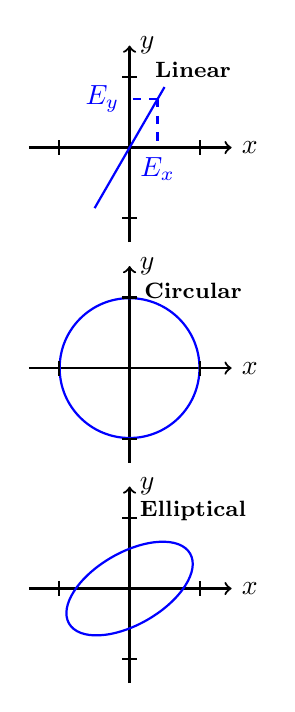
\begin{tikzpicture}[scale=0.8]
  \def\xmax{6.5}         % max x axis
  \def\ymin{-1.5}        % min y axis
  \def\ymax{1.6}         % max y axis
  \def\zmax{1.6}         % max z axis
  \def\xf{1.17*\xmax}    % x position frequency axis
  \def\A{(0.70*\ymax)}   % amplitude
  \def\T{(0.335*\xmax)}  % period
  \def\w{\zmax/11.2}     % spacing components
  \def\ang{60}           % angle
  \def\s{\ang/360*\T}    % time component
  \def\x{\A*cos(\ang)}   % real component
  \def\y{\A*sin(\ang)}   % imaginary component

  \tikzstyle{vector}=[->,very thick,black!50]
  \tikzstyle{xline}=[blue,thick]
  \def\tick#1#2{\draw[thick] (#1) ++ (#2:0.12) --++ (#2-180:0.24)}

  % LINEAR POLARISATION PLANE
  \begin{scope}
    \draw[->,thick] (0,\ymin) -- (0,\ymax+0.02)
    node[right] {$y$};
    \draw[->,thick] (-\zmax,0) -- (\zmax+0.02,0)
    node[right] {$x$};
    \draw[xline,rotate=60] ({-0.991*\A},0) -- ({0.991*\A},0) coordinate[pos=0.9] (end);
    \draw[draw,blue,thick,dashed] (end) -- (0,0 |- end) node[left] {$E_y$};
    \draw[draw,blue,thick,dashed] (end) -- (end |- 0,0) node[below] {$E_x$};
    \node at ({0.9*\A},{1.1*\A}) {\footnotesize\textbf{Linear}};
    \tick{{\A},0}{90};
    \tick{{-\A},0}{90};
    \tick{0,{\A}}{0};
    \tick{0,{-\A}}{0};
  \end{scope}

  % CIRCULAR POLARISATION PLANE
  \begin{scope}[yshift=-3.5cm]
    \draw[->,thick] (0,\ymin) -- (0,\ymax+0.02)
    node[right] {$y$};
    \draw[->,thick] (-\zmax,0) -- (\zmax+0.02,0)
    node[right] {$x$};
    \draw[xline] (0,0) circle(0.991*\A);
    \node at ({0.9*\A},{1.1*\A}) {\footnotesize\textbf{Circular}};
    \tick{{\A},0}{90};
    \tick{{-\A},0}{90};
    \tick{0,{\A}}{0};
    \tick{0,{-\A}}{0};
  \end{scope}

  % ELLIPTICAL POLARISATION PLANE
  \begin{scope}[yshift=-7.0cm]
    \draw[->,thick] (0,\ymin) -- (0,\ymax+0.02)
    node[right] {$y$};
    \draw[->,thick] (-\zmax,0) -- (\zmax+0.02,0)
    node[right] {$x$};
    \draw[xline,rotate=30] (0,0) ellipse({0.991*\A} and {0.51*\A});
    \node at ({0.9*\A},{1.1*\A}) {\footnotesize\textbf{Elliptical}};
    \tick{{\A},0}{90};
    \tick{{-\A},0}{90};
    \tick{0,{\A}}{0};
    \tick{0,{-\A}}{0};
  \end{scope}
\end{tikzpicture}
